\documentclass[12pt,a4paper,oneside]{book} 

%%%%%%%%%%%%%%%%%%%%%%%%%%%%%%%%%%%%%

\usepackage{ifthen}
\usepackage{graphicx}
\usepackage[dvips]{epsfig}
\usepackage{enumerate}
\usepackage{calc}
\usepackage{multicol} 
\usepackage{titlesec}
%\usepackage{showkeys}

%%%%%%%%%%%%%%%%%%%%%%%%%%%%%%%%%%%%%

\usepackage{a4}
\usepackage{amsfonts}
\usepackage{amssymb}
\usepackage{epsfig}

%%%%%%%%%%%%%%%%%%%%%%%%%%%%%%%%%%%%%%

\usepackage{t1enc,times}
\usepackage{latexsym,amssymb}
\usepackage{amsmath}
\usepackage{amstext}
%\usepackage[T1]{fontenc}
%\usepackage{cmbright}
\usepackage{pifont}
\usepackage{marvosym}
%\usepackage{pslatex}
% \usepackage{stmaryrd} %=== > dont have it installed on system, 
% doesnt look like it's a compulsory package anyway
%\usepackage{txfonts}  

%%%%%%%%%%%%%%%%%%%%%%%%%%%%%%%%%%%%%%

\usepackage[titletoc]{appendix}
\usepackage{mathrsfs}

%%%%%%%%%%%%%%%%%%%%%%%%%%%%%%%%%%%

\usepackage{fancybox} 
\usepackage{fancyhdr}
\usepackage{fullpage}

%%%%%%%%%%%%%%%%%%%%%%%%%%%%%%%%%%%

%\usepackage{url}    
%\ExecuteOptions{dvips}
%\usepackage[pdftex,colorlinks=true]{hyperref}
%\hypersetup{backref,pdfpagemode=UseThumbs,pdfstartview=Fit,
%pdfpagelayout=SinglePage,pdfstartpage=1,colorlinks=true,menucolor=msc,
%anchorcolor=msc,pagecolor=msc,urlcolor=rfr,breaklinks=true,hyperfootnotes=true}

%%%%%%%%%%%%%%%%%%%%%%%%%%%%%%%%%%%%

\pagestyle{fancy}
\fancyhf{} 
%\renewcommand{\headrulewidth}{1pt}
%\renewcommand{\footrulewidth}{1pt}
\renewcommand{\headwidth}{\textwidth}
\fancyhead[LE]{\leftmark}
\fancyhead[RO]{\small \rightmark}
\fancyfoot[C]{\thepage}

%%%%%%%%%%%%%%%%%%%%%%%%%%%%%%%%%%%%

\tolerance 4000
\textwidth 17.00cm
\topmargin -0.30cm
\oddsidemargin -0.25cm
\evensidemargin -0.25cm
\textheight 23.00cm
%\headsep 12pt
\headheight 15pt
\footskip 60pt
%\parindent 12pt

%%%%%%%%%%%%%%%%%%%%%%%%%%%%%%%%%%%%

\renewcommand{\rmdefault}{ptm}  % times
\renewcommand{\rmdefault}{phv}  % helvetica
\renewcommand{\rmdefault}{pbk}  % bookman
\renewcommand{\rmdefault}{ppl}  % palatino
\renewcommand{\sfdefault}{phv}  % helvetica as sans serif
\renewcommand{\ttdefault}{pcr}  % courier as fixed width
\renewcommand{\tabcolsep}{8pt}
\renewcommand{\arraystretch}{1.25}

%%%%%%%%%%%%%%%%%%%%%%%%%%%%%%%%%%%%

\newcommand{\Lim}[1]{\raisebox{0.5ex}{\scalebox{0.8}{$\displaystyle \lim_{#1}\;$}}}

%%%%%%%%%%%%%%%%%%%%%%%%%%%%%%%%%%%%

\def\nn{\nonumber}
\def\f{{\frac}}
\def\pa{{\partial}}
\def\d{{\rm d}}
\def\l{\left}
\def\r{\right}
\def\Mpl{M_{_{\rm Pl}}}

%%%%%%%%%%%%%%%%%%%%%%%%%%%%%%%%%%%%

\def\done{\marginpar {\scriptsize DONE}}
\def\check{\marginpar {\scriptsize CHECK}}

%%%%%%%%%%%%%%%%%%%%%%%%%%%%%%%%%%

\begin{document}

%%%%%%%%%%%%%%%%%%%%%%%%%%%%%%%%%%%

\baselineskip 20pt

%%%%%%%%%%%%%%%%%%%%%%%%%%%%%%%%%%%

\pagenumbering{roman}

%%%%%%%%%%%%%%%%%%%%%%%%%%%%%%%%%%%

\thispagestyle{empty}
\topskip 15pt
\hrule\hrule\hrule\hrule\hrule
\vskip 20pt
\centerline{\Huge \bf Numerical evaluation of the} 
\vskip 15pt
\centerline{\Huge \bf tensor bi-spectrum during inflation}
\vskip 20pt
\hrule\hrule\hrule\hrule\hrule
\vskip 30pt
\centerline{\Large A project report}
\vskip 8pt
\centerline{\Large submitted in partial fulfilment 
for the award of the degree of}
\vskip 8pt
\centerline{\Large B.S \& M.S in Physics}
%\vskip 8pt
%\centerline{\Large in}
%\vskip 8pt 
%\centerline{\Large Physics}
\vskip 8pt
\centerline{\Large by}
\vskip 8pt
\centerline{\Large \bf Poruri Sai Rahul}
\vskip 8pt
\centerline{\Large under the guidance of}
\vskip 8pt
\centerline{\Large  Dr.~L.~Sriramkumar}
\vskip 30pt 
\begin{center}

\epsfig{file=iitm.eps, width=3.0cm, height=3.0cm}
% needed to convert .ps ext to .eps ext.
\end{center}
\vskip 8pt 
\centerline{\Large \bf Department of Physics}
\vskip 8pt 
\centerline{\Large \bf Indian Institute of Technology Madras}
\vskip 8pt 
\centerline{\Large \bf Chennai~600036, India}
\vskip 8pt
\centerline{\Large \bf June~2015}
%%%%%%%%%%%%%%%%%%%%%%%%%%%%%%%%%%%%

\newpage\topskip 40pt
\centerline{\Large CERTIFICATE}
\thispagestyle{empty}
\vskip 20pt\noindent 
This is to certify that the project titled {\bf Numerical evaluation 
of the tensor bi-spectrum during power law inflation} is a bona fide 
record of work done by {\bf Poruri Sai Rahul} towards the partial fulfilment 
of the requirements of the B.S \& M.S degree in Physics at the Indian 
Institute of Technology, Madras, Chennai 600036, India.
\vskip 120pt
\hspace{240pt}(L.~Sriramkumar, Project supervisor)

%%%%%%%%%%%%%%%%%%%%%%%%%%%%%%%%%%%%%%%%

\newpage\topskip 40pt
\thispagestyle{empty}
\centerline{\Large ACKNOWLEDGEMENTS}
\vskip 20pt\noindent 

I cannot express in words my gratitude to {\bf Dr. L.~Sriramkumar} for 
guiding me, regarding my work and my personal life. I would also like to 
thank V.~Sreenath and Debika Choudhury for helping me with my project 
and for clarifying my doubts. I would like to thank my family and my 
friends, especially Preeti Saryan and Malayaja Chutani, who have kept 
me on my toes over the last few years.
 
 %%%%%%%%%%%%%%%%%%%%%%%%%%%%%%%%%%%%%%%%

\newpage\topskip 40pt
\thispagestyle{empty}
\centerline{\Large ABSTRACT}
\vskip 20pt\noindent 

\paragraph*{} Theories of inflation provide a causal mechanism for the 
origin of perturbations in the early universe, perturbations which evolve and 
leave an imprint on the cosmic microwave background (CMB). The n-point 
statistics of the observed perturbations can be used to constrain various models 
of inflation. In this work, I study 
the tensor bi-spectrum during two models of inflation, namely during 
power law inflation and during inflation driven by a quadratic potential model. 
The aim of this work 
is to construct a Python code to numerically evaluate the tensor bi-spectrum 
during inflation for an arbitrary triangular configuration of wavevectors.

%%%%%%%%%%%%%%%%%%%%%%%%%%%%%%%%%%%%%%%%%

\newpage
\thispagestyle{empty}
\tableofcontents
\newpage

%%%%%%%%%%%%%%%%%%%%%%%%%%%%%%%%%%%%%%%%%

\newpage
\thispagestyle{empty}
\listoffigures
\newpage

%%%%%%%%%%%%%%%%%%%%%%%%%%%%%%%%%%%%%%%%%

\pagenumbering{arabic}

%%%%%%%%%%%%%%%%%%%%%%%%%%%%%%%%%%%%%

\chapter{Introduction}

\paragraph*{} Inflation refers to a period of rapid expansion in the early 
universe and the theory of inflation was proposed to overcome a few of the drawbacks 
of the conventional hot big bang model of the universe, the flatness problem 
and the horizon problem to name a few. Inflation also provides a causal mechanism 
for the generation of perturbations in the universe, perturbations which evolved 
into the large scale structure of the universe. From an observational perspective, 
the inhomogenities in the early universe leave an imprint on the CMB and studying 
the CMB will help us constrain numerous inflationary models, specifically, 
the n-point statistics of perturbations. The two-point statistic refers to the 
power spectrum of perturbations and the three-point statistic refers to the bi-spectrum 
of perturbations. In this work, I will study with the tensor bi-spectrum, the easiest of the 
three-point functions.
%While CMBR observations by the Wilkinson Microwave 
%Anisotropy Probe (WMAP) \cite{WMAP} and Planck \cite{Planck} can be used to estimate the n-point statistics 
%of scalar perturbations, CMBR polarization observations such as those made by BICEP, 
%Keck array estimate the n-point statistics of tensor perturbations. 


\paragraph*{} This thesis presents a study of the tensor bi-spectrum $G({\bf k}_1, {\bf k}_2, {\bf k}_3)$ and the 
non-Gaussianity parameter $h_{NL}$. In this chapter, I give a brief introduction to 
inflation and why scalar fields are needed to drive inflation. I also introduce the 
conditions imposed on a scalar field that drives inflation. I will also discuss linear 
perturbation theory and tensor perturbations in the metric. I 
will discuss how the scale factor, $a(t)$, the scalar field, $\phi$, and the potential 
driving the scalar field, $V(\phi)$, are related to each other. In the next chapter, I will discuss 
how we can solve the equation governing tensor perturbations after we obtain 
solutions for the scalar field driving inflation. After solving for the tensor perturbations, 
I will discuss how the tensor bi-spectrum, $G({\bf k}_1, {\bf k}_2, {\bf k}_3)$, can be evaluated using the solutions 
we obtained earlier for the 
tensor perturbations. In the third chapter, I will discuss the numerical methods 
implemented to solve for the scalar field $\phi$, the tensor perturbations $h_k$, 
the tensor bi-spectrum $G({\bf k}_1, {\bf k}_2, {\bf k}_3)$ and the non-Gaussianity parameter $h_{NL}$.

\section{Conventions and notations}

\paragraph*{} I shall work in $(3+1)$ dimensions  and I shall adopt the metric 
signature $(+,-,-,-)$. Latin indices, with the exception of $k$ which represents 
wavevectors, represent spatial 
coordinates whereas greek indices denote all spacetime coordinates. Planck 
mass is defined as $M_{Pl} = (8\pi G)^{-1/2}$. 
$t$ refers to cosmic time and an overdot refers to differentiation 
with respect to cosmic time whereas $\eta$ refers to conformal time and an 
overprime represents differentiation with respect to conformal time. For convenience 
with the numerics, we measure the duration of inflation not in terms of cosmic time 
or conformal time but in terms of e-folds $N$, where $N$ is defined as

\begin{equation}
N = {\rm ln}\left(\frac{a(t)}{a_0}\right),
\end{equation}

\noindent $a_0$ is the scale factor when inflation started and $a(t)$ is the scale factor 
when inflation ends.

\section{Metric perturbations}

\paragraph*{} Inhomogenities in the Cosmic Microwave Background 
have been measured to be one part in $10^5$ and given the expanding 
nature of our universe, it can be inferred that they were much smaller 
at earlier epochs. Therefore, we can study the generation and evolution 
of such anisotropies in the universe using linear perturbation theory.

\paragraph*{} The perturbations in a Friedmann background can be 
classified as scalar, vector and tensor according to their behaviour under 
local rotation of spatial coordinates on hyper surfaces of constant time. 
The perturbations that remain invariant under rotations are classified as 
scalar. In fact, scalar perturbations are largely responsible for the anisotropy 
we see in our universe. Vector and tensor perturbations behave as vectors and 
tensors under local rotations. Rotational velocity fields generate vector perturbations 
and are therefore also referred to as Vorticity modes and 
the tensor perturbations describe gravitational waves. (In this context, see refs. 
\cite{Sriramkumar L - 2009, Dodelson, Durrer, Riotto, Kinney, Linde, B1, B2, G1, AG} 
can be studied for a better understanding of cosmological linear perturbation theory.)
I shall restrict myself to tensor perturbations of the metric for the scope of this work.

\paragraph*{} The metric tensor governing a Friedmann universe describes a 
homogeneous and isotropic universe, which is not a valid assumption under the presence 
of perturbations. We can therefore choose to work in a number of coordinate systems 
under the condition that they reduce to the standard Friedmann line element in the limit 
when the perturbations vanish. A particular choice of coordinates is referred to as a gauge 
and a gauge transformation refers to the transformation from one gauge to another. 
We can therefore choose to work with quantities that are gauge-invariant or work in a 
specific gauge throughout. We adopt the latter approach. We shall represent the tensor 
perturbations in the metric as 

\begin{equation}\label{eq:tensormetric}
{\rm d}s^2 = {\rm d}t^2 - a^2(t)(\delta_{ij} + h_{ij}){\rm d}x^i{\rm d}x^j,
\end{equation}

\noindent where the tensor perturbations are characterized by the transverse, traceless 
matrix $h_{ij}$ and $h_{ii}=0$ \& $\delta_i h_{ij}=0$. % and $\delta_{ij}$ is a $4\times 4$ Identity matrix.

\paragraph*{} Similar to how we characterized the perturbations, we can 
characterize the sources which give rise to them, namely the stress-energy 
tensor. Like the metric tensor, the stress-energy tensor is a two tensor and 
therefore, perturbations in the stress-energy tensor can also be classified into 
scalar, vector and tensor components. The decomposition theorem dictates  
that scalar, vector and tensor perturbations are decoupled and can therefore 
be studied independent of one another. Therefore, a scalar field driving inflation is a scalar 
source that gives rise to scalar perturbations, 
velocity fields with Vorticity are vector sources that give rise to vector perturbations 
and having eliminated the scalar and vector contributions, anisotropic stresses constitute a tensor 
source that give rise to tensor perturbations.

\paragraph*{} The perturbed metric, say $\delta g_{\mu\nu}$, can be used to 
derive the perturbed Einstein tensors, which can then be related to the 
perturbed stress-energy tensor, say $\delta T_{\mu\nu}$, giving rise to 
the Einstein's equations which govern the evolution of the metric perturbations. 

\paragraph*{} Under these assumptions, the perturbed Einstein tensors 
corresponding to the metric described in Eqn. (\ref{eq:tensormetric}) are 
given by

\begin{equation}
\delta G^0_0 = \delta G^0_i = 0,
\end{equation}

\begin{equation}
\delta G^i_j = -\left(\frac{1}{2}\right)\left(\ddot{h}_{ij} + 3H\dot{h}_{ij} 
- \frac{1}{a^2}\nabla ^2h_{ij}\right),
\end{equation}

\noindent after imposing the condition that $h_{ij}$ is a transverse and traceless matrix. 
%Similarly, the perturbed stress-energy tensor can be written 
%in terms of it's individual components as

%\begin{equation}
%\delta T^0_0 = \delta\rho,
%\end{equation}

%\begin{equation}
%\delta T^0_i = \left(\nabla_i\delta\sigma\right),
%\end{equation}

%\begin{equation}
%\delta T^i_j = -\delta p~\delta^i_j.
%\end{equation}

%\noindent where $\rho$ is the energy density and $p$ is the pressure of the source 
%of perturbations.

\paragraph*{} In the absence of anisotropic stresses i.e if $\delta T^i_j = 0$
, we get that

\begin{equation}\label{eq:tensor_perturbation_ODE}
\ddot{h} + 3H\dot{h} - \left(\frac{1}{a^2}\right)\nabla ^2h = 0.
\end{equation}

\noindent which is the equation governing the evolution of tensor 
perturbations across cosmic time $t$. The above equation 
can be rewritten in terms of conformal time $\eta$ as 

\begin{equation}\label{eq:tensor_perturbation_ODE_eta}
{h}^{''} + 2{\mathcal{H}}{h}^{'} - \nabla ^2h = 0,
\end{equation}

\noindent where ${\mathcal{H}} = a^{'}/a$.

\section{Quantization of perturbations}

\paragraph*{} Eqn. (\ref{eq:tensor_perturbation_ODE_eta}) can be 
rewritten in fourier space as 

\begin{equation}\label{eq:tensor_perturbation_eqn_fourier}
h_k^{''} + 2{\mathcal{H}}h_k^{'} + k^2	h_k = 0.
\end{equation}

\paragraph*{} The homogeneity of the Friedmann background allows us 
to quantize the tensor perturbations. Upon quantization, we can write the 
tensor perturbation $\hat{h}$ in terms of it's fourier component 
$h_k(\eta)$ as 

\begin{equation}\label{eq:quantization_tensor_perturbation}
\hat{h}(\eta, {\bf x}) = \sum_s \int \frac{{\rm d}^3\bf{k}}{(2\pi)^{3/2}} 
\left[\hat{a_k}^s\varepsilon^{s}_{ij}({\bf k})h_k(\eta)e^{i\bf{k\cdot x}}
+\hat{a_k}^{s^{\dagger}}\varepsilon^{s*}_{ij}({\bf k})h_k^{*}(\eta)e^{-i\bf{k\cdot x}}\right] ,
\end{equation}

\noindent where the creation and annihilation operators, $\hat{a}_k$ and $\hat{a}_k^{\dagger}$, 
follow the standard commutation relations. As we are working in the linear 
order in perturbations, the two point function of the quantum field $\hat{h}$ 
can be used to characterize the power spectrum of the tensor perturbations. 
The power spectrum of the tensor perturbations $\mathcal{P}_T(k)$ and the 
two point function are related by

\begin{equation}\label{eq:estimation_power_spectrum_fourier}
\int^{\infty}_0 {\rm d}k ~{\mathcal{P}}_{\rm T}(k) = \int {\rm d}^3
{\bf{k}}\int\frac{{\rm d}^3(\bf{x}-\bf{x'})}{(2\pi)^3}~\langle 0|\hat{h}
(\eta,{\bf{x}})\hat{h}(\eta, {\bf{x'}})|0\rangle ~e^{-i{\bf{k \cdot (x-x')}}},
\end{equation}

\noindent where $|0\rangle$ is the vacuum state defined as 
$\hat{a_{\bf k}}|0\rangle = 0 ~\forall ~{\bf k}$. 
Using Eqs. (\ref{eq:tensor_perturbation_eqn_fourier}) and 
(\ref{eq:quantization_tensor_perturbation}), we can obtain 
the tensor power spectrum as

\begin{equation}\label{eq:tensor_power_spectrum}
{\mathcal{P}}_{\rm T}(k) = 2 \left(\frac{k^3}{2\pi^2}\right) |h_k|^2,
\end{equation}

\noindent where the factor of 2 is needed to take into account the two 
states of polarization, $+$ and $\times$, of the gravitational waves.

\section{The Bunch-Davies initial conditions}

\paragraph*{} We need to understand the initial conditions from which the 
tensor perturbations evolve in order to arrive at a complete analytical 
solution to the problem at hand. On individual modes, we impose the 
initial conditions when they are well within the Hubble radius i.e when 
$\eta \rightarrow -\infty$ or $(k/aH) >> 1$. In this sub-Hubble limit, the curvature 
of spacetime can be neglected. Further, upon imposing the condition that the 
solution $u_k$ contain positive frequency modes, we obtain a solution to the 
Eqn. (\ref{eq:tensor_perturbation_ODE_mod}) in the sub-Hubble limit as 

\begin{equation}\label{eq:bunch_davies}
\Lim{\left(k/aH\right) \rightarrow \infty} u_k(\eta) \rightarrow 
\left(\frac{1}{\sqrt{2k}}\right){\rm e}^{-ik\eta}.
\end{equation}

\section{Tensor bi-spectrum}

\paragraph*{} The moments of primordial perturbations can be used to understand 
their statistical properties. The variance or the power spectrum of the primordial 
perturbations would have contained all of it's statistical properties if they were Gaussian. 
However, non-Gaussianities in the primordial perturbations would manifest either as 
non-zero odd moments or as the even moments taking a different form. Hence, non-zero 
three point functions of the primordial perturbations would be the first evidence of 
non-Gaussianity. We adopt the so-called Maldacena formalism as it is the most complete 
formalism to calculate the three-point functions generated during inflation amongst 
different approaches \cite{Maldacena}. In this section, we will only concentrate on the 
three-point function involving tensors.

\paragraph*{} The tensor bi-spectrum in Fourier space, 
$G_{\gamma\gamma\gamma}^{m_1n_1m_2n_2m_3n_3}({\bf k}_1, {\bf k}_2, {\bf k}_3)$ 
evaluated towards the end of 
inflation at conformal time, say $\eta_e$, is defined as \cite{Maldacena, 31, 32, Pi-1, Pi-2}

\begin{equation}
\langle\hat{\gamma}^{{\bf k}_1}_{m_1n_1}(\eta_e)\hat
{\gamma}^{{\bf k}_2}_{m_2n_2}(\eta_e)\hat
{\gamma}^{{\bf k}_3}_{m_3n_3}(\eta_e)\rangle = 
 (2\pi)^{-3/2}G_{\gamma\gamma\gamma}^{m_1n_1m_2n_2m_3n_3}({\bf k}_1, {\bf k}_2 {\bf k}_3)
 \delta^{(3)}({\bf k}_1+{\bf k}_2+{\bf k}_3)
\end{equation}

\noindent where ${\gamma}^{{\bf k}}_{mn}$ represents the tensor perturbation ${\gamma}_{mn}$ 
in Fourier space.

\paragraph*{} We can arrive at the tensor three-point function using the action governing the 
tensor perturbations and the standard rules of perturbative quantum field theory \cite{Maldacena, 31, 32, Pi-1, Pi-2}. 
Using Maldecena's approach, we can obtain a cubic order action of the form,

\begin{equation}
S^{3}_{\gamma\gamma\gamma}[\gamma_{ij}] = \frac{1}{2}
\int{\rm d}\eta\int{\rm d^3}{\bf x}
\left[\frac{a^2}{2}\gamma_{lj}\gamma_{im}\partial_l\partial_m\gamma_{ij}
-\frac{a^4}{4}\gamma_{ij}\gamma_{lm}\partial_l\partial_m\gamma_{ij}\right]
\end{equation}

\paragraph*{} The interaction Hamiltonian corresponding to the above action is needed 
to evaluate the three-point correlation function using the methods 
of quantum field theory. At the cubic order, it can be shown that 
$H_{int} = -L_{int}$, where $H_{int}$ is the 
interaction Hamiltonian and $L_{int}$ is the interaction Lagrangian \cite{Maldacena, 31, 32, Pi-1, Pi-2}.
The tensor bi-spectrum $G_{\gamma\gamma\gamma}^{m_1n_1m_2n_2m_3n_3}({\bf k}_1, {\bf k}_2, {\bf k}_3)$
can be expressed in terms of the Hamiltonian $\hat{H}_{\gamma\gamma\gamma}$ as \cite{32, Pi-2, 56}

\begin{equation}
\langle\hat{\gamma}^{{\bf k}_1}_{m_1n_1}(\eta_e)\hat
{\gamma}^{{\bf k}_2}_{m_2n_2}(\eta_e)\hat
{\gamma}^{{\bf k}_3}_{m_3n_3}(\eta_e)\rangle = 
-i\int_{\eta_i}^{\eta_e} {\rm d}\eta 
\langle[\hat{\gamma}^{{\bf k}_1}_{m_1n_1}(\eta_e)\hat
{\gamma}^{{\bf k}_2}_{m_2n_2}(\eta_e)\hat
{\gamma}^{{\bf k}_3}_{m_3n_3}(\eta_e),
\hat{H}_{\gamma\gamma\gamma}(\eta)]\rangle
\end{equation}

\paragraph*{} The tensor bi-spectrum $G_{\gamma\gamma\gamma}^{m_1n_1m_2n_2m_3n_3}({\bf k}_1, {\bf k}_2, {\bf k}_3)$,
calculated in perturbative vaccum, can be written as \cite{Maldacena, 32, Pi-2, 56}

\begin{align*}\label{eq:G}
& G_{\gamma\gamma\gamma}^{m_1n_1m_2n_2m_3n_3}({\bf k}_1, {\bf k}_2, {\bf k}_3) = \\
& M_{Pl}^2\left[\left(
\Pi^{{\bf k}_1}_{m_1n_1,ij}\Pi^{{\bf k}_2}_{m_2n_2,im}\Pi^{{\bf k}_3}_{m_3n_3,lj} 
-\frac{1}{2}\Pi^{{\bf k}_1}_{m_1n_1,ij}\Pi^{{\bf k}_2}_{m_2n_2,ml}\Pi^{3}_{m_3n_3,ij}
\right)k_{1m}k_{1l} + {\rm five} {\rm permutations}\right]\\
& \times\left[h_{k1}(\eta_e)h_{k2}(\eta_e)h_{k3}(\eta_e)\mathcal{G}_{\gamma\gamma\gamma} 
+{\rm complex conjugate}\right]
\end{align*}

\noindent where the quantities $\mathcal{G}$ and $\Pi^{{\bf k}}_{ij,mn}$ is 
given by \cite{Pi-1, Pi-2}

\begin{equation}\label{eq:calG}
\mathcal{G}_{\gamma\gamma\gamma}({\bf k}_1, {\bf k}_2, {\bf k}_3) = 
\frac{-i}{4}\int^{\eta_e}_{\eta_i}{\rm d}\eta a^2 h_{{\bf k}_1}^*h_{{\bf k}_2}^*h_{{\bf k}_3}^*,
\end{equation}

\begin{equation}
\Pi^{{\bf k}}_{ij,mn}= \sum_{s} \varepsilon^s_{ij}({\bf k})\varepsilon^{s*}_{mn}({\bf k})
\end{equation}

\noindent where the quantity $\varepsilon^s_{ij}({\bf k})$ represents the polarization 
tensor of gravitational waves with helicity $s$. The condition 
$\varepsilon^s_{ii}({\bf k}) = {\bf k}_i\varepsilon^s_{ij}({\bf k}) = 0$ can be arrived at given the 
traverse, traceless nature of the tensor perturbations $h_{ij}$. %Also note that we work 
%with the normalization condition $\varepsilon^r_{ij}(\vec{k})\varepsilon^{s*}_{ij}(\vec{k}) = 2\delta^{rs}$
%\cite{Maldacena}. 
It is to be noted that we had neglected the polarization tensor earlier 
in estimating the tensor power spectrum earlier and 
that we will not be including it in our numerical procedure.
It should also be noted that $(k_{1i}, k_{2i}, k_{3i})$ denote the components of the wavevectors 
$({\bf k}_1, {\bf k}_2, {\bf k}_3)$ along the i-spatial direction.

\section{Driving inflation}

\paragraph*{} In a spatially flat, smooth Friedmann universe, the line 
element is described by

\begin{equation}
{\rm d}s^2 = {\rm d}t^2 - a^2(t){\rm d}{\bf x}^2 = 
a^2(\eta)\left({\rm d}\eta^2 - {\rm d}{\bf x}^2\right),
\end{equation}

\noindent and for such a line element, the Einstein's equations can be rewritten as 
the following two Friedmann equations

\begin{equation}\label{eq:friedmann1}
\left(\frac{\dot{a}}{a}\right)^2 = H^2 = 
\left(\frac{8\pi G}{3}\right)\rho,
\end{equation}

\begin{equation}\label{eq:friedmann2}
\left(\frac{\ddot{a}}{a}\right) = \dot{H} + H^2= 
-\left(\frac{4\pi G}{3}\right)(\rho + 3p),
\end{equation}

\noindent where $\rho$ and $p$ denote the energy density and the pressure of the 
field driving the change and $H=\dot{a}/a$ is the Hubble parameter.

\paragraph*{} A necessary condition to solve the horizon problem and to achieve 
inflation on the scale factor $a(t)$ is 

\begin{equation}\label{eq:ddot_a}
\ddot{a} > 0.
\end{equation}

\paragraph*{} From Eqns. (\ref{eq:friedmann2}) and (\ref{eq:ddot_a}), it 
is straight forward to notice that 

\begin{equation}
(\rho + 3p) < 0,
\end{equation}

\noindent is a necessary condition for a field that drives inflation. We know that a matter 
field has $p=0$ and that a radiation field has $p=\rho/3$, neither of which 
satisfy the above condition. We therefore invoke the presence of a scalar field $\phi$, 
itself driven by a potential $V(\phi)$, to drive inflation. A scalar field that drives 
inflation is also referred to as an Inflaton.

\paragraph*{} We can write the action, $S[\phi]$, for such a scalar field 
and the corresponding stress-energy tensor $T_{\mu\nu}$ as

\begin{equation}\label{eq:action}
S[\phi] = \int {\rm d}^4x \sqrt{-g}\left[ \left(\frac{1}{2}\right)
\left(\partial^{\lambda}\phi \partial_{\lambda}\phi\right) - V(\phi)\right],
\end{equation}

\begin{equation}\label{eq:stress_energy_tensor}
T^{\mu}_{\nu} = \partial^{\mu}\phi \partial_{\nu}\phi 
-\delta^{\mu}_{\nu}\left[\left(\frac{1}{2}\right)
\left(\partial^{\lambda}\phi \partial_{\lambda}\phi\right) - V(\phi)\right].
\end{equation}

\paragraph*{} From Eqn. (\ref{eq:action}) defining the action, $S[\phi]$, for a scalar 
field $\phi$, we can derive the equation of motion for the scalar field to be

\begin{equation}\label{eq:phi_ODE}
\ddot{\phi} + 3H\dot{\phi} + V_{\phi} = 0,
\end{equation}

\noindent where $V_{\phi} = {\rm d}V/{\rm d}\phi$.

\paragraph*{} We can also arrive at solutions to the scalar field, $\phi$, and the 
potential, $V(\phi)$, using the stress-energy tensor, $T^{\mu}_{\nu}$, 
defined in Eqn. (\ref{eq:stress_energy_tensor}) 
and the Friedmann equations defined in Eqns. (\ref{eq:friedmann1}) and (\ref{eq:friedmann2}). 
From Eqn. (\ref{eq:stress_energy_tensor}), we can 
write the individual components of the stress-energy tensor as 

\begin{equation}\label{eq:stress_energy_00}
T^{0}_{0} = \left(\frac{\dot{\phi}^2}{2}\right) +V(\phi) = \rho,
\end{equation}

\begin{equation}\label{eq:stress_energy_ij}
T^{i}_{j} = -\left[\left(\frac{\dot{\phi}^2}{2}\right) - V(\phi)\right]\delta^{i}_{j} = -p\delta^i_j.
\end{equation}

\paragraph*{} Using the definitions for energy density $\rho$ and the pressure 
$p$ from Eqs. (\ref{eq:stress_energy_00}) and (\ref{eq:stress_energy_ij}), 
we can rewrite Eqs. (\ref{eq:friedmann1}) and (\ref{eq:friedmann2}) defining the 
Hubble parameter and the evolution of the Hubble parameter in cosmic time $t$ as

\begin{equation}\label{eq:dH_vs_dphi}
 \dot{H} = \frac{-\dot{\phi}^2}{2M_{Pl}^2},
\end{equation}

\begin{equation}\label{eq:Hubble_parameter}
H^2 = \left(\frac{1}{3M_{Pl}^2}\right)\left(\frac{\dot{\phi}^2}{2} + V\right).
\end{equation}

\paragraph*{} We can now express the scalar field $\phi$ and the 
potential $V$ in terms of cosmic time ${\rm t}$ as

\begin{equation}\label{eq:phi_vs_H}
\phi(t)= \sqrt{2}\int dt \sqrt{-\dot{H}},
\end{equation}

\begin{equation}\label{eq:V_vs_H}
V(t) = 3H^2 + \dot{H}.
\end{equation}


%%%%%%%%%%%%%%%%%%%%%%%%%%%%%%%%%%%%%%%

\chapter{Inflationary models}

\section{Power law inflation}

\subsection{Inflaton}

\paragraph*{} Power law inflation is one of many models of inflation where
inflation is being driven by a single scalar field. During power law inflation, 
we assume that the scale factor, $a(t)$, has a power law dependence on 
cosmic time $t$, namely 

\begin{equation}\label{eq:a_power_law}
a(t) = a_0t^q.
\end{equation}

\noindent which can be rewritten in terms 
of conformal time $\eta$ as 

\begin{equation}
a(\eta) = \left(-\mathcal{\bar{H}}\eta\right)^{\left(\gamma+1\right)},
\end{equation}

\noindent where $\mathcal{\bar{H}}$ and $\gamma$ are given by 

\begin{equation}
\mathcal{\bar{H}} = a_0^{1/q}(q-1) ~{\rm ~and}~ \gamma  = -\left(\frac{2q-1}{q-1}\right).
\end{equation}

\paragraph*{} Using the scale factor given by Eqn. (\ref{eq:a_power_law}), 
we can rewrite the Eqns. (\ref{eq:phi_vs_H}) and (\ref{eq:V_vs_H}) that define 
the scalar field, $\phi$, and the potential, $V$, as

\begin{equation}
\phi(t) =\sqrt{\left(2q\right)} ~{\rm ln}\left[t\sqrt
{\left(\frac{V_0}{(3q-1)q}\right)}\right],
\end{equation}

\begin{equation}
V(\phi) = V_0~\exp\left[-\phi\sqrt{\left(\frac{2}{q}\right)}\right].
\end{equation}

\paragraph*{} Further, for convenience in numerical evaluation, we can rewrite 
the scalar field, $\phi$, and the Hubble parameter, $H$, in terms of e-fold $N$ as 

\begin{equation}
\phi(N) = \sqrt{\left(\frac{2}{q}\right)} N 
- \sqrt{\left(2q\right)}~{\rm ln}~t_0.
\end{equation}

\begin{equation}
H(N) = H_0\exp^{-N/q}.
\end{equation}

\noindent where $t_0 = \sqrt{\left((3q-1)q/V_0\right)}$

%\begin{equation}
%\epsilon_1(N) = \frac{1}{2}\left(\frac{{\rm d}\phi}{{\rm d} N}\right)^2 
%= \frac{1}{q},
%\end{equation}

\paragraph*{} Having solved the background equations, we can now 
attempt to solve the equation governing the tensor perturbations. We can 
rewrite Eqn. (\ref{eq:tensor_perturbation_ODE_eta}) governing the evolution 
of tensor perturbations in conformal time, $\eta$, by substituting 
$h_k = \left(u_k/a\right)$ as

\begin{equation}\label{eq:tensor_perturbation_ODE_mod}
u''_k + \left[k^2 - \left(\frac{a''}{a}\right)\right]u_k = 0,
\end{equation}

\noindent and the power spectrum governing tensor perturbations, namely 
Eqn. (\ref{eq:tensor_power_spectrum}), can be rewritten as

\begin{equation}
{\mathcal{P}}_{\rm T}(k) = 2 \left(\frac{k^3}{2\pi^2}\right) |h_k|^2 
= 2 \left(\frac{k^3}{2\pi^2}\right) \left(\frac{|u_k|}{a}\right)^2.
\end{equation}

\subsection{Tensor power spectrum}

\paragraph*{} Armed with the analytic solutions to the background driving 
inflation and the initial conditions imposed on the tensor perturbations, we 
can attempt to solve the Eqn. (\ref{eq:tensor_perturbation_eqn_fourier}) 
governing the evolution of tensor perturbations in fourier space to obtain 
the power spectrum of tensor perturbations. 
Substituting the scale factor given by Eqn. (\ref{eq:a_power_law}) 
in the Eqn. (\ref{eq:tensor_perturbation_ODE_mod}), we can arrive at a solution 
satisfying the initial conditions defined in Eqn. (\ref{eq:bunch_davies}) as 

\begin{equation}\label{eq:u_k_solution}
u_k(\eta) = \left(\frac{-\pi\eta}{4}\right)^{1/2}{\rm e}^{i[\nu+(1/2)]
(\pi/2)}{\rm H}_{\nu}^{(1)}(-k\eta),
\end{equation}

\noindent where $\nu = [\gamma + (1/2)]$ and ${\rm H}_{\nu}^{(1)}$ is the 
Hankel function of the first kind and of order $\nu$ (Ref. \cite{Ab}). In the 
super-Hubble limit $($ i.e as $(-k\eta \rightarrow 0))$, 
we can approximate the Hankel function to

\begin{equation}
{\rm H}_{\nu}^{(1)}(z) \sim -(i/\pi)\Gamma(\nu)\left(\frac{z}{2}\right)^{(-\nu)}.
\end{equation}

\noindent where $\Gamma(\nu)$ is a Gamma function.

\paragraph*{} In the super-Hubble limit, $u_k$ and $a$ have the same 
behaviour and therefore, the tensor perturbation $h_k$ reach a constant value, 
allowing us to obtain the tensor power spectrum in the super-Hubble limit as 

\begin{equation}
\mathcal{P}_{\rm T}(k) = 
A_T\bar{\mathcal{H}}^2\left(\frac{k}{\mathcal{\bar{H}}}\right)^{2(\gamma+2)},
\end{equation}

\noindent where

\begin{equation}
A_T = \left[\frac{1}{\pi^3}\right]
\left(\frac{|\Gamma(\nu)|^2}{2^{(2\gamma+1)}}\right).
\end{equation}

\section{Slow roll inflation}

\paragraph*{} We have previously seen that $(\rho + 3p) < 0$ is a necessary condition 
for inflation to take place. Using the definitions of $\rho$ and $p$ from Eqn. (\ref{eq:stress_energy_00})
 and Eqn. (\ref{eq:stress_energy_ij}), we can restate the above the condition as 
$\dot{\phi}^2<V(\phi)$. However, if $\dot{\phi}^2<<V(\phi)$, Inflation is guaranteed 
to take place. We can interpret the above condition as the field slowly rolling 
down the potential, $V(\phi)$. Moreover, using the above condition and 
Eqn. (\ref{eq:phi_ODE}), we can ensure that inflation occurs for a sufficiently 
long time, provided $\ddot{\phi}<<3H\dot{\phi}$. These two conditions 
on the first and second derivative of the scalar field, $phi$, lead to the slow-roll 
approximation, using which we can construct analytical solutions for the evolution 
of the background and the evolution of tensor perturbations.

\paragraph*{} The slow-roll condition is quantified using slow-roll parameters and 
two types of slow-roll parameters are often considered in literature, namely 
potential slow-roll parameters and Hubble slow-roll parameters. We will only be 
working with the Hubble slow-roll parameters.

\paragraph*{} The Eqn. (\ref{eq:dH_vs_dphi}) can be rewritten as 

\begin{equation}\label{eq:dphi_Hphi}
\dot{\phi} = -2M_{Pl}^2H_{\phi},
\end{equation}

\noindent where $H_{\phi} = {\rm d}H/{\rm d}\phi$. This expression can be used to rewrite 
the Eqn. (\ref{eq:Hubble_parameter}) as 

\begin{equation}\label{eq:HJI}
H_{\phi}^2 - \frac{3H^2}{2M_{Pl}^2} = -\frac{V}{2M_{Pl}^4},
\end{equation}

\noindent which 

\paragraph*{} The above equation is referred to as the Hamilton-Jacobi formulation of inflation. 
Considering the Hubble parameter, $H$, to be a function of the scalar field, $\phi$, we can 
define the dimensionless Hubble slow-roll parameters $\varepsilon_H$ and $\delta_H$ as 

\begin{equation}
\varepsilon_H = 2M_{Pl}^2\left(\frac{H_{\phi}}{H}\right)^2
\delta_H = 2M_{Pl}^2\left(\frac{H_{\phi\phi}}{H}\right)
\end{equation}

\noindent where ${\rm d}^2H/{\rm d}\phi^2$. Using Eqns. (\ref{eq:phi_ODE}), (\ref{eq:dphi_Hphi})
 and (\ref{eq:HJI}), we can rewrite the two Hubble slow-roll parameters as 
 
 \begin{equation}
 \varepsilon_H = -\left(\frac{\dot{H}}{H^2}\right),
 \delta_H = \varepsilon_H - \left(\frac{\dot{\varepsilon_H}}{2H\varepsilon_H}\right).
 \end{equation}

\paragraph*{} Note that conditions on the Hubble slow-roll parameters $\varepsilon_H$ and $\delta_H$ 
correspond to constraining the kinetic energy of the scalar field and the acceleration of the scalar field, 
respectively. Specifically, kinetic energy of the scalar field can be neglected if $\varepsilon_H<<1$ and 
the acceleration of the scalar field can be ignored in comparison to the term involving the 
velocity, $\dot{\phi}$, if $\delta_H<<1$.

\subsection{Inflation}

\paragraph*{} Using the above definitions of the slow-roll parameters, let us now arrive at an 
analytic solution to the evolution of the scalar field. We can rewrite Eqn. (\ref{eq:phi_ODE}), 
the equation governing the evolution of the scalar field. and Eqn. (\ref{eq:Hubble_parameter}) 
in terms of the slow-roll parameters as 

\begin{equation}
H^2\left(1-\frac{\varepsilon_H}{3}\right) = \frac{V}{3M_{Pl}^2},
3H\dot{\phi}\left(1-\frac{\delta_H}{3}\right) = -V_{\phi}.
\end{equation}

\paragraph*{} In the slow-roll approximation, $\varepsilon_H<<1$ and $\delta_H<<1$, 
the above equations can be rewritten as 

\begin{equation}
H^2 = \frac{V}{3M_{Pl}^2},
3H\dot{\phi} = -V_{\phi}.
\end{equation}

\paragraph*{} The above equations can be integrated trivially to arrive at an analytic 
solutions to evolution of the scalar field, $\phi$. We can look at a general set of models 
the potential, $V(\phi)$, where is defined as $V(\phi) = V_0\phi^n$. These set of models 
are classified as `large-field' models. For such as form of the potential function, the 
analytic solution to the scalar field is given by 

\begin{equation}
\phi^{(4-n)/2)}(t) = \phi^{(4-n)/2)}_i + \sqrt{\frac{V_0}{3}}\left(\frac{n(n-4)}{2}\right)M_{Pl}(t-t_i),
\phi(t) = phi_i\exp^{-\sqrt{V_0/3}4M_{Pl}(t-t_i)}.
\end{equation}

\noindent where the first solution is when $n \neq 4$ and the second when $n = 4$.

\subsection{Tensor power spectrum}

\paragraph*{} The two Hubble slow-roll parameters, $\varepsilon_H$ and $\delta_H$,  
can be rewritten in terms of the conformal time coordinate, $\eta$, as 

\begin{equation}\label{eq:calH_eta}
\varepsilon_H = 1-\left(\frac{\mathcal{H'}}{\mathcal{H}^2}\right),
\delta_H = \varepsilon_H - \left(\frac{\varepsilon_H'}{2\mathcal{H}\varepsilon_H}\right).
\end{equation}

\paragraph*{} Further, using the first Hubble slow-roll parameter, $\varepsilon_H$, 
we can establish that

\begin{equation}\label{eq:a''/a}
\left(\frac{a''}{a}\right) = \mathcal{H}^2(2-\varepsilon_H).
\end{equation}

\paragraph*{} In order to arrive at an analytic solution to the evolution 
of tensor perturbations, we need to solve Eqn. (\ref{eq:tensor_perturbation_ODE_mod}). 
In order to do so, we need to represent $\mathcal{H}$, in terms of $\eta$.

\paragraph*{} In order to arrive at an analytic solution to the evolution of the 
tensor perturbations using the Eqn. (\ref{eq:tensor_perturbation_ODE}), 
we need to be able to write $\mathcal{H}$ in terms of conformal time $\eta$. 
We can rewrite the first of the two equations in Eqn. (\ref{eq:calH_eta}) as 

\begin{equation}
\eta = -\int \left(\frac{1}{1-\varepsilon_H}\right){\rm d}\left(\frac{1}{\mathcal{H}}\right),
\end{equation}

\paragraph*{} Under the slow-roll approximation, $\varepsilon_H<<1$, the above 
integral becomes trivial and leads to 

\begin{equation}
\mathcal{H} = - \left[\frac{1}{(1-\varepsilon_H})\eta\right]
\end{equation}

\paragraph*{} Using the above expression for $\mathcal{H}$ in terms of the conformal time, 
$\eta$, we can rewrite the Eqn. (\ref{eq:a''/a}) as 

\begin{equation}
\left(\frac{a''}{a}\right) = \left(\frac{2+3\varepsilon_H}{\eta^2}\right)
\end{equation}

\noindent where we assumed the slow-roll approximation and 
neglected the higher orders of $\varepsilon_H$.

\paragraph*{} We can now solve the Eqn. (\ref{eq:tensor_perturbation_ODE_mod}). We can 
clearly see that the solutions to the equation will be Hankel functions \cite{DLMF}, similar to 
the solutions in the power law case, of order, $\nu$,

\begin{equation}
\nu = \left[\left(\frac{3}{2}\right)+\varepsilon_H\right]
\end{equation}

\paragraph*{} The tensor power spectrum can now be evaluated in the super-Hubble limit, 
i.e $-k\eta\rightarrow 0$, by expanding the Hankel function about the origin, as

\begin{equation}\label{eq:tps_slowroll}
\mathcal{P}_T(k) = \left(\frac{2H^2}{\pi^2M_{Pl}^2}\right)
\left[\frac{|\Gamma(\nu)|}{\Gamma(3/2)}\right]^2 2^{(2\nu-3)}(1-\varepsilon_H)^{(2\nu-1)}
\end{equation}

\noindent where we assumed that $-k\eta = (1-\varepsilon_H)^{-1}$. In the slow-roll approximation, 
the tensor power spectrum at the leading order can be approximated as 

\begin{equation}
\mathcal{P}_T(k) = \left(\frac{8}{2M_{Pl}^2}\right)\left(\frac{H}{2\pi}\right)^2_{k=aH}.
\end{equation}

\noindent evaluated when the modes cross the Hubble radius.

\subsection{Tensor bi-spectrum}

\paragraph*{} Having defined the tensor bi-spectrum, let us evaluate the tensor 
bi-spectrum in slow roll inflation. The first two slow roll parameters, namely 
$\epsilon_1$ and $\epsilon_2$, are constant at the leading order in the slow 
approximation. We can assume that the scale factor as well as the tensor perturbation 
mode, $h_k$, are given by their de Sitter forms. By setting the slow roll parameters in 
the index, $\nu$, of the Hankel function to zero, we 
can obtain the de Sitter limit of the tensor perturbation modes as

\begin{equation}
h_k(\eta) = \frac{\sqrt{2}}{M_{Pl}}\frac{iH_0}{\sqrt{2k^3}}(1+ik\eta)e^{-ik\eta}
\end{equation}

\paragraph*{} The tensor bi-spectrum can now be estimated by simply 
substituting the above form of $h_k$ and evaluating the integral in Eqn. (\ref{eq:calG}) 
from $\eta_i = -\infty$ to $\eta_e = 0$.

\begin{align*}
& \mathcal{G}_{\gamma\gamma\gamma}({\bf k}_1, {\bf k}_2, {\bf k}_3) = 
\frac{-i}{4}\frac{1}{H_0^2}\left(\frac{-iH_0}{M_{Pl}}\right)^3 \frac{1}{\sqrt{k_1^3k_2^3k_3^3}} 
\int^{\eta_e}_{\eta_i}{\rm d}\eta \frac{1}{\eta^2}(1-ik_1\eta)(1-ik_2\eta)(1-ik_3\eta)e^{ik_T\eta} \\
& =  \frac{-i}{4}\frac{1}{H_0^2}\left(\frac{-iH_0}{M_{Pl}}\right)^3 \frac{1}{\sqrt{k_1^3k_2^3k_3^3}}
 \int^{\eta_e}_{\eta_i}{\rm d}\eta \frac{1}{\eta^2}\left[-1+ik_T\eta +(k_1k_2 +k_2k_3 +k_3k_1)\eta^2 -ik_1k_2k_3\eta^3\right]e^{ik_T\eta}
\end{align*}

\noindent where $k_T = k_1 +k_2 +k_3$. As you can see, the above integrand can be separated into four terms 
with different powers of $\eta$. While the $\eta^0$ and $\eta^1$ are straight forward to integrate, it should 
be noted that the $\eta^{-2}$ and $\eta^{-1}$terms should be integrated together, giving rise to a term similar 
to$e^{-\eta}/\eta$. Together with the complex conjugate term, this term can be converted into a 
$\sin \eta/\eta$ term and set to $1$. We can finally obtain the tensor bi-spectrum to be 

\begin{align*}
& G_{\gamma\gamma\gamma}^{m_1n_1m_2n_2m_3n_3}({\bf k}_1, {\bf k}_2, {\bf k}_3) = \\
& \frac{H_0^4}{2M_{Pl}^4}\frac{1}{k_1^3k_2^3k_3^3}
\left[\left(
\Pi^{\vec{k_1}}_{m_1n_1,ij}\Pi^{\vec{k_2}}_{m_2n_2,im}\Pi^{\vec{k_3}}_{m_3n_3,lj} 
-\frac{1}{2}\Pi^{\vec{k_1}}_{m_1n_1,ij}\Pi^{\vec{k_2}}_{m_2n_2,ml}\Pi^{\vec{k_3}}_{m_3n_3,ij}
\right)k_{1m}k_{1l} + {\rm five} {\rm permutations}\right]\\
& \times\left[-k_T +\frac{k_1k_2 +k_2k_3 + k_3k_1}{k_T} + \frac{k_1k_2k_3}{k_T^2}\right]
\end{align*}

%%%%%%%%%%%%%%%%%%%%%%%%%%%%%%%%%%%

\chapter{Numerical results}

I shall now discuss the numerical methods used to evaluate the scalar field,
the tensor power spectrum and the tensor bi-spectrum during two models 
of inflation, namely power law inflation and inflation driven by a quadratic potential 
model. The chapter is split into three sections on Inflation, Tensor power spectrum 
and Tensor bi-spectrum. Each section is further split into two subsections where I 
shall discuss the numerical results for power law inflation and for inflation driven by 
a quadratic potential model. Also, as the Tensor bi-spectrum is evaluated in three 
limits, namely in the equilateral limit, in the squeezed limit and for an arbitrary configuration 
of wavevectors, the section on Tensor bi-spectrum is divided as such, in which 
the numerical results for power law inflation and for inflation driven by quadratic 
potential model will be discussed.
%Note that we are working in units of $M_{\rm Pl}=1$.

\section{Inflaton}

\subsection{Power law inflation}

As mentioned earlier, the scalar field driving the inflation is often referred to as the `Inflation'. 
We assume that the potential $V(\phi)$ driving inflation is related to the scalar field $\phi$ as 

\begin{equation}\label{eq:vofphi}
V(\phi) = V_0 \exp\left[-\sqrt{\frac{2}{q}}\left(\phi - \phi_i\right)\right],
\end{equation}

\noindent where $\phi_i$ is the value of the scalar field at $N=0$ and $q$ is the power law index. 
Recall that the equation governing the scalar field is given by 

\begin{equation}\label{eq:phi_ODE}
\ddot{\phi} + 3H\dot{\phi} + V_{\phi} = 0,
\end{equation}

\noindent where $V_{\phi} = {\rm d}V/{\rm d}\phi$. 
We shall now rewrite the above equation in terms of e-fold $N$ as

\begin{equation}\label{eq:phi_ODE_N}
\frac{{\rm d}^2\phi}{{\rm d}N^2} + \left[3 - \frac{1}{2}\left(\frac{{\rm d}\phi}
{{\rm d}N}\right)^2\right]\frac{{\rm d}\phi}{{\rm d}N} + \left[6 
- \left(\frac{{\rm d}\phi}{{\rm d}N}\right)^2\right]\frac{1}{2V(\phi)}
\frac{{\rm d}V(\phi)}{{\rm d}N} = 0.
\end{equation}

\noindent Note that the the Hubble parameter $H$ in the above equation is defined as

\begin{equation}
H^2 = \frac{2V(\phi)}{3-({\rm d}\phi/{\rm d}N)^2}.
\end{equation}

\paragraph*{} We numerically solve the Eqn. (\ref{eq:tensor_perturbations_ODE_N}) using an implementation 
of the fourth order Runge-Kutta method in Python \cite{python, numpy, matplotlib}. Integration is performed from 
e-fold $N = 0$  to $N = 70$. Note that the initial conditions for solving the differential equation are 

\begin{equation}
\phi = 1,
\end{equation}

\begin{equation}
\frac{{\rm d}\phi}{{\rm d}N} = \left(\frac{\sqrt{2q}}{t_0}\frac{1}{H_0}\right),
\end{equation}

\noindent where $H_0$ is the value of the Hubble parameter at $N=0$. 
Also note that $\phi$ at $N=0$ was referred to as $\phi_i$ in Eqn.(\ref{eq:vofphi})

\begin{figure}
\begin{center}
\includegraphics[scale=0.6]{plots/power_law/phi_vs_N.png}
\caption[Plot of $\phi(N)$ as a function of $N$ in power law inflation.]
{Plot of $\phi(N)$ as a function of $N$.}
\label{fig:field_vs_N}
\end{center}
\end{figure}

\begin{figure}
\begin{center}
\includegraphics[scale=0.6]{plots/power_law/H_vs_N.png}
\caption[Plot of $H(N)$ as a function of $N$ in power law inflation.]
{Plot of $H(N)$ as a function of $N$.}
\label{fig:Hubble_vs_N}
\end{center}
\end{figure}

\paragraph*{} Figures \ref{fig:field_vs_N} and \ref{fig:Hubble_vs_N} show the numerical estimates 
of the scalar field $\phi$ and the Hubble parameter $H$ as a function of e-fold time $N$.

\subsection{Quadratic potential model}

\paragraph*{} The potential driving inflation in the quadratic potential model is 

\begin{equation}\label{eq:vofphi_quad}
V(\phi) = \frac{1}{2}m^2\phi^2,
\end{equation}

\noindent where $m = 7147\times 10^{-9}$.

\paragraph*{} We arrive at a numerical solution for the scalar field during inflation driven 
by quadratic potential model in the same manner with which we arrived at the numerical results 
in the previous case, during power law inflation. We numerically solved the Eqn. (\ref{eq:phi_ODE_N}) 
using a Runge-Kutta 4 method implemented in python. To arrive at the numerical solution, we assumed 
that the initial values for the scalar field, $phi$, and it's derivative with respect to e-fold $N$, ${\rm d}\phi/{\rm d}N$ as 

\begin{equation}
\phi = \frac{165}{10},
\end{equation}

\begin{equation}
\frac{{\rm d}\phi}{{\rm d}N} = -10^{-5}.
\end{equation}

\paragraph*{} Figure \ref{fig:field_vs_N_quad} shows the numerical estimate of the scalar 
field with respect to e-fold $N$ and Figure \ref{fig:Hubble_vs_N_quad} shows the numerical 
estimate of the Hubble parameter, $H$, with respect to e-fold $N$ during inflation 
driven by a quadratic potential model.

\begin{figure}
\begin{center}
\includegraphics[scale=0.6]{plots/quadratic_potential/phi_vs_N.png}
\caption[Plot of $\phi(N)$ as a function of $N$ in quadratic potential model.]
{Plot of $\phi(N)$ as a function of $N$.}
\label{fig:field_vs_N_quad}
\end{center}
\end{figure}

\begin{figure}
\begin{center}
\includegraphics[scale=0.6]{plots/quadratic_potential/H_vs_N.png}
\caption[Plot of $H(N)$ as a function of $N$ in quadratic potential model.]
{Plot of $H(N)$ as a function of $N$.}
\label{fig:Hubble_vs_N_quad}
\end{center}
\end{figure}

\section{Tensor power spectrum}

\subsection{Power law inflation}

\paragraph*{} The Eqn. (\ref{eq:tensor_perturbation_ODE}) governing the evolution 
of tensor perturbations in cosmic time $t$ can be rewritten in terms of e-fold $N$ as 

\begin{equation}\label{eq:tensor_perturbations_ODE_N}
\frac{{\rm d}^2h_k}{{\rm d}N^2} +\left (3+\frac{1}{H}\frac{{\rm d}H}
{{\rm d}N}\right)\frac{{\rm d}h_k}{{\rm d}N} + \frac{k^2}{a^2H^2}h_k = 0.
\end{equation}

\paragraph*{} We can now solve the above second order differential equation numerically 
as we already have the numerical solution of the scalar field, $\phi$, and Hubble parameter, $H$, 
as functions of e-fold $N$. Similar to the integration routine used to numerically estimate the 
scalar field $\phi$, we use a fourth order Runge-Kutta method to solve the above equation numerically.

\paragraph*{} To arrive at the initial conditions to perform the numerical integration, we first need
to arrive at an appropriate e-fold $N$. In our results, we choose to set the initial conditions 
when the modes are well inside the Hubble scale corresponding to the mode i.e $k/aH = 100$. 
We perform the numerical integration till e-fold $N$ when the modes are well outside the 
Hubble radius i.e $k/aH = 10^{-5}$. Using the Bunch-Davies initial conditions, Eqn. (\ref{eq:bunch_davies}), 
we can write $h_k$ and ${\rm d}h_k/{\rm d}N$ in terms of e-fold $N$ as 

\begin{equation}\label{eq:h_k_init}
h_k  = \frac{1}{\sqrt{2k_0}a(N)},
\end{equation}

\begin{equation}\label{eq:Dh_k_init}
\frac{{\rm d}h_k}{{\rm d}N} = -\frac{1}{\sqrt{2k_0}a(N)} - \frac{i\sqrt{(k_0/2)}}{a^2(N)H(N)},
\end{equation}

\paragraph*{} From the numerical solution to $h_k$, we can evaluate the tensor power spectrum using Eqn. (\ref{eq:tensor_power_spectrum}).
Figure \ref{tps_p} shows the numerical solution of the tensor power spectrum $\mathcal{P}_T(k)$ as a function of $k$.

\begin{figure}
\begin{center}
\includegraphics[scale=0.6]{plots/power_law/tps_vs_k.png}
\caption[Plot of $\mathcal{P}_{\rm T}(k)$ as a function of $k$ in power law inflation.]
{Plot of $\mathcal{P}_{\rm T}(k)$ as a function of $k$.}
\label{tps_p}
\end{center}
\end{figure}

\subsection{Quadratic potential model}

\paragraph*{} Having arrive at the numerical solution for the background driving tensor 
perturbations during inflation driven by a quadratic potential model, we can now solve 
the Eqn. (\ref{eq:tensor_perturbations_ODE_N}) to arrive at a numerical solution for the 
evolution of the tensor perturbations. Again, as mentioned earlier in the case for power law 
inflation, we assume that the initial conditions for tensor perturbations, $h_k$,  and the 
derivative of the tensor perturbations with respect to e-fold $N$, ${\rm d}h_k/{\rm d}N$, 
using the Eqns. (\ref{eq:h_k_init}) and (\ref{eq:Dh_k_init}).

\paragraph*{} Figure \ref{tps_p_quad} shows a numerical solution for the 
power spectrum of tensor perturbations in the super-Hubble limit during inflation 
driven by a quadratic potential model.

\begin{figure}
\begin{center}
\includegraphics[scale=0.6]{plots/quadratic_potential/tps_vs_k.png}
\caption[Plot of $\mathcal{P}_{\rm T}(k)$ as a function of $k$ in quadratic potential model.]
{Plot of $\mathcal{P}_{\rm T}(k)$ as a function of $k$.}
\label{tps_p_quad}
\end{center}
\end{figure}

\section{Tensor bi-spectrum}

\paragraph*{} As mentioned earlier, we neglect the polarization of the tensor perturbations. 
We can therefore rewrite the Eqn. (\ref{eq:G}) that defines tensor bi-spectrum, $G$, and 
the non-gaussianity parameter $h_{NL}$ as 

\begin{equation}\label{eqn:G_eta}
G = h_{k_1}(\eta_e)h_{k_2}(\eta_e)h_{k_3}(\eta_e)\mathcal{G} 
	+h_{k_1}^{*}(\eta_e)h_{k_2}^{*}(\eta_e)h_{k_3}^{*}(\eta_e)\mathcal{G}^{*}
\end{equation}

\noindent where

\begin{equation}\label{eqn:calG_eta}
\mathcal{G} = \frac{-i}{4}(k_1^2+k_2^2+k_3^2)\int^{\eta_e}_{\eta_i} {\rm d}\eta a(\eta) h_{k_1}^{*}(\eta)h_{k_2}^{*}(\eta)h_{k_3}^{*}(\eta)
\end{equation}

\paragraph*{} 

\begin{equation}\label{eqn:h_NL_eta}
h_{NL} = \frac{k_1^3k_2^3k_3^3G}
{k_1^3\mathcal{P}_{T}(\eta_e)\mathcal{P}_{T}(\eta_e)
+ k_2^3\mathcal{P}_{T}(\eta_e)\mathcal{P}_{T}(\eta_e)
+ k_3^3\mathcal{P}_{T}(\eta_e)\mathcal{P}_{T}(\eta_e)}
\end{equation}

\paragraph*{} While the equations governing the tensor bi-spectrum, $G$, 
and the non-gaussianity parameter, $h_{NL}$, can be trivially converted from 
cosmic time $t$ to e-fold $N$, the integral $\mathcal{G}$ can be rewritten as 

\begin{equation}\label{eqn:calG_N}
\mathcal{G} = \frac{-i}{4}(k_1^2+k_2^2+k_3^2)\int^{N_f}_{N_i} {\rm d}N \frac{a(N)}{H(N)} h_{k_1}^{*}(N)h_{k_2}^{*}(N)h_{k_3}^{*}(N)
\end{equation}

\paragraph*{} It is to be noted that the function, $h_k$, and therefore the integral itself 
oscillate highly in the extreme sub-Hubble domain ($k\eta\rightarrow -\infty$). In order to 
regulate these integrals, we introduce a cut-off factor $e^{-\kappa k_T/3a(N)H(N)}$, where 
$\kappa$ is a small positive quantity and $k_T$ is the sum of the individual wavevectors. 
Such a cut-off also proves to be essential inorder to identify the correct perturbative vaccum.

\subsection{Equilateral limit}

\begin{equation}
k^6G_{\gamma\gamma\gamma}(k) \propto k^{4(\Gamma+2)}
\end{equation}

\begin{equation}
k_1^3k^3G_{\gamma\gamma\gamma}^{m_1n_1m_2n_2m_3n_3}(k_1,k) \propto k_1^{2(\gamma+2)}k^{2(\gamma+2)}
\end{equation}

\begin{equation}
\gamma = -\left(\frac{2q-1}{q-1}\right)
\end{equation}

\subsubsection{Power law inflation}

\paragraph*{} In the equilateral limit, we assume that the three wavevectors, $k_1, k_2$ and $k_3$, 
have the same amplitude. We can therefore rewrite Eqn. (\ref{eq:calG}) as 

\begin{equation}\label{eqn:calG_N_eq}
\mathcal{G} = \frac{-i}{4}(3k^2)\int^{N_f}_{N_i} {\rm d}N \frac{a(N)}{H(N)} h_{k}^{*}(N)^3
\end{equation}

\paragraph*{} We can solve the above integral as we already have the numerical solutions of the scale 
factor $a(N)$, the Hubble parameter $H(N)$ and the strength of tensor perturbations $h_k(N)$. We 
evaluate the integrals over the same limits in which we solved the Eqn. (\ref{eq:tensor_perturbations_ODE_N}), 
i.e from when the modes are well inside the Hubble scale corresponding to the mode i.e $k/aH = 100$ till 
when the modes are well outside the Hubble radius i.e $k/aH = 10^{-5}$.

\paragraph*{} Figure \ref{fig:eq_calG_vs_k} shows the dependence of $\mathcal{G}$ on the amplitude of the 
wavevector $k$.

\begin{figure}
\begin{center}
\includegraphics[scale=0.6]{plots/power_law/calG_vs_k.png}
\caption[Plot of $\mathcal{G}(k)$ as a function of $k$ in the equilateral limit in power law inflation.]
{Plot of $\mathcal{G}(k)$ as a function of $k$ in the equilateral limit.}
\label{fig:eq_calG_vs_k}
\end{center}
\end{figure}

\paragraph*{} Figure \ref{fig:eq_G_vs_k} 
shows the numerical estimate of the Tensor Bi-Spectrum $G$ as a function of $k$. Given the dependence 
of $h_k$ and $\mathcal{G}$ on $k$, we can arrive at the fact that $k^6G$ is an invariant quantity. The figure 
\ref{fig:eq_k6G_vs_k} shows the invariance of $k^6G$ as a function of $k$.

\begin{figure}
\begin{center}
\includegraphics[scale=0.6]{plots/power_law/G_vs_k.png}
\caption[Plot of $G(k)$ as a function of $k$ in the equilateral limit in power law inflation.]
{Plot of $G(k)$ as a function of $k$ in the equilateral limit.}
\label{fig:eq_G_vs_k}
\end{center}
\end{figure}

\begin{figure}
\begin{center}
\includegraphics[scale=0.6]{plots/power_law/k6G_vs_k.png}
\caption[Plot of $k^6G(k)$ as a function of $k$ in the equilateral limit in power law inflation.]
{Plot of $k^6G(k)$ as a function of $k$ in the equilateral limit.}
\label{fig:eq_k6G_vs_k}
\end{center}
\end{figure}

\paragraph*{} We can finally estimate the value of the non-gaussianity parameter $h_{NL}$ using Eqn. (\ref{eqn:h_NL_eta}). 
Figure \ref{fig:eq_h_NL_vs_k} shows the dependence of $h_{NL}$ as a function of $k$. As you can see, the value of the 
$h_{NL}$ is invariant in $k$.

\begin{figure}
\begin{center}
\includegraphics[scale=0.6]{plots/power_law/h_NL_vs_k.png}
\caption[Plot of $h_{NL}$ as a function of $k$ in the equilateral limit in power law inflation.]
{Plot of $h_{NL}$ as a function of $k$ in the equilateral limit.}
\label{fig:eq_h_NL_vs_k}
\end{center}
\end{figure}

\subsubsection{Quadratic potential model}

\paragraph*{} Having arrived at a numerical solution for the evolution of tensor 
perturbations during inflation driven by quadratic potential earlier, we can now evaluate 
the tensor bi-spectrum numerically. Again, as in the case with power law inflation earlier, 
we solve the Eqn. (\ref{eqn:calG_N_eq}) numerically to arrive at the integral $\mathcal{G}$ 
using which we can arrive at the tensor bi-spectrum, $G$, and the non-gaussianity parameter, 
$h_{NL}$.

\paragraph*{} Figure \ref{fig:eq_calG_vs_k_quad} shows the numerical solution to the integral $\mathcal{G}$ 
with respect to e-fold wavenumber $k$. Figure \ref{fig:eq_G_vs_k_quad} shows the numerical solution to the 
tensor bi-spectrum $G$ as a function wavenumber $k$. Figure \ref{fig:eq_k6G_vs_k_quad} shows the 
invariance of $k^6G$ with respect to $k$ and Figure \ref{fig:eq_h_NL_vs_k_quad} shows the numerical 
solution of the non-gaussianity parameter, $h_{NL}$, with respect to wavenumber $k$.

\begin{figure}
\begin{center}
\includegraphics[scale=0.6]{plots/quadratic_potential/calG_vs_k.png}
\caption[Plot of $\mathcal{G}(k)$ as a function of $k$ in the equilateral limit in quadratic potential model.]
{Plot of $\mathcal{G}(k)$ as a function of $k$ in the equilateral limit.}
\label{fig:eq_calG_vs_k_quad}
\end{center}
\end{figure}

\begin{figure}
\begin{center}
\includegraphics[scale=0.6]{plots/quadratic_potential/G_vs_k.png}
\caption[Plot of $G(k)$ as a function of $k$ in the equilateral limit in quadratic potential model.]
{Plot of $G(k)$ as a function of $k$ in the equilateral limit.}
\label{fig:eq_G_vs_k_quad}
\end{center}
\end{figure}

\begin{figure}
\begin{center}
\includegraphics[scale=0.6]{plots/quadratic_potential/k6G_vs_k.png}
\caption[Plot of $k^6G(k)$ as a function of $k$ in the equilateral limit in quadratic potential model.]
{Plot of $k^6G(k)$ as a function of $k$ in the equilateral limit.}
\label{fig:eq_k6G_vs_k_quad}
\end{center}
\end{figure}

\begin{figure}
\begin{center}
\includegraphics[scale=0.6]{plots/quadratic_potential/h_NL_vs_k.png}
\caption[Plot of $h_{NL}$ as a function of $k$ in the equilateral limit in quadratic potential model.]
{Plot of $h_{NL}$ as a function of $k$ in the equilateral limit.}
\label{fig:eq_h_NL_vs_k_quad}
\end{center}
\end{figure}

\subsection{Squeezed limit}

\subsubsection{Power law inflation}

\paragraph*{} In the squeezed limit, we assume that the amplitude of two of the modes is equal, say $|k_1|=|k_2|= |k|$ 
and we assume $k_3$ to be a pseudo-zero mode, $k_0$, with an amplitude much smaller than $k$. We numerically arrive 
at the solutions of $k$ and $k_0$ independently following which we evaluate the integral in $\mathcal{G}$ from $\eta_i$ 
corresponding to the smallest mode, $k_0$, till $\eta_e$ corresponding to the largest mode, $k$.

\paragraph*{} Figure \ref{fig:sq_G_vs_k} shows the numerical estimate of the Tensor Bi-spectrum value $G$ as a function of $k$ 
in the squeezed limit and figure \ref{fig:sq_k6G_vs_k} shows the invariance of $k^{3/2}k_0^{3/2}G$. 

\begin{figure}
\begin{center}
\includegraphics[scale=0.6]{plots/power_law/G_vs_k_sq.png}
\caption[Plot of $G(k)$ as a function of $k$ in the squeezed limit in power law inflation.]
{Plot of $G(k)$ as a function of $k$ in the squeezed limit.}
\label{fig:sq_G_vs_k}
\end{center}
\end{figure}

\begin{figure}
\begin{center}
\includegraphics[scale=0.6]{plots/power_law/k6G_vs_k_sq.png}
\caption[Plot of $k_0^{3/2}k^{3/2}G(k)$ as a function of $k$ in the squeezed limit in power law inflation.]
{Plot of $k_0^{3/2}k^{3/2}G(k)$ as a function of $k$ in the squeezed limit.}
\label{fig:sq_k6G_vs_k}
\end{center}
\end{figure}

\paragraph*{} Figure \ref{fig:sq_h_NL_vs_k} shows the numerical estimate of the 
non-gaussianity parameter $h_{NL}$ as a function of $k$ in the squeezed limit and 
as you can see, $h_{NL}$ reaches an invariant value.

\begin{figure}
\begin{center}
\includegraphics[scale=0.6]{plots/power_law/h_NL_vs_k_sq.png}
\caption[Plot of $h_{NL}$ as a function of $k$ in the squeezed limit in power law inflation.]
{Plot of $h_{NL}$ as a function of $k$ in the squeezed limit.}
\label{fig:sq_h_NL_vs_k}
\end{center}
\end{figure}

\subsubsection{Quadratic potential model}

\paragraph*{} As mentioned earlier, when we estimated the tensor bi-spectrum 
in the squeezed limit during power law inflation, we set $|k_1|=|k_2|=|k|$ and 
we $|k_3|=|k_0|$, where $|k|>>|k_0|$. Using the above assumption and 
the numerical solutions to the tensor perturbations for various $k$, we first 
arrive at a numerical estimate of the integral, $\mathcal{G}$, using which we 
can estimate the tensor bi-spectrum, $G$, and the non-Gaussianity parameter, $h_{NL}$, 
as a function of wavenumber $k$.

\paragraph*{} Figure \ref{fig:sq_G_vs_k_quad} shows the numerical estimate of the 
tensor bi-spectrum during inflation driven by a quadratic potential model and Figure 
\ref{fig:sq_k6G_vs_k_quad} shows the invariance of $k^3Gk_0^3G$ with respect to 
the wavenumber $k$ in the squeezed limit. Figure \ref{fig:sq_h_NL_vs_k_quad} shows 
the numerical estimate of the non-Gaussianity parameter, $h_{NL}$, with respect to $k$.

\begin{figure}
\begin{center}
\includegraphics[scale=0.6]{plots/quadratic_potential/G_vs_k_sq.png}
\caption[Plot of $G(k)$ as a function of $k$ in the squeezed limit in quadratic potential model.]
{Plot of $G(k)$ as a function of $k$ in the squeezed limit.}
\label{fig:sq_G_vs_k_quad}
\end{center}
\end{figure}

\begin{figure}
\begin{center}
\includegraphics[scale=0.6]{plots/quadratic_potential/k6G_vs_k_sq.png}
\caption[Plot of $k_0^{3/2}k^{3/2}G(k)$ as a function of $k$ in the squeezed limit in quadratic potential model.]
{Plot of $k_0^{3/2}k^{3/2}G(k)$ as a function of $k$ in the squeezed limit.}
\label{fig:sq_k6G_vs_k_quad}
\end{center}
\end{figure}

\begin{figure}
\begin{center}
\includegraphics[scale=0.6]{plots/quadratic_potential/h_NL_vs_k_sq.png}
\caption[Plot of $h_{NL}$ as a function of $k$ in the squeezed limit in quadratic potential model.]
{Plot of $h_{NL}$ as a function of $k$ in the squeezed limit.}
\label{fig:sq_h_NL_vs_k_quad}
\end{center}
\end{figure}

\subsection{Triangular configuration of wavevectors}

\subsubsection{Power law inflation}

\paragraph*{} In this case, we consider wavevectors, $k_1, k_2$ and $k_3$ which form 
a triangle. Numerically speaking, we fix $|k_1| = 1e-02$ and we vary 
$|k3|$ from $0$ till $1e-02$. From these two values and the fact that 

\begin{equation}
|k_1|^2+|k_2|^2+|k_3|^2 = 1
\end{equation}

\noindent we can estimate the value of $|k2|$. We solve the Eqn. (\ref{eq:tensor_perturbations_ODE_N}) 
to find the numerical solutions to this triangular configuration of wavevectors. Numerically, we solve 
the Eqn. (\ref{eq:tensor_perturbations_ODE_N}) from $N_i$ corresponding to the smallest wavevector a
till $N_f$ corresponding to the largest wavevector where $N_i$ and $N_f$ are e-fold $N$ 
when the modes are well inside the Hubble scale corresponding to the mode i.e $k/aH = 100$ and
when the modes are well outside the Hubble radius i.e $k/aH = 10^{-5}$.

\paragraph*{} Figure \ref{fig:tr_h_NL_vs_k} shows the $h_{NL}$ values for such a triangular configuration 
of wavevectors.

\begin{figure}
\begin{center}
\includegraphics[scale=0.6]{plots/power_law/h_NL_tr_lt.png}
\caption[Plot of $h_{NL}$ as a function of $k$ for a triangular configuration of wavevectors in power law inflation.]
{Plot of $h_{NL}$ as a function of $k$ for a triangular configuration of wavevectors.}
\label{fig:tr_h_NL_vs_k}
\end{center}
\end{figure}

\subsubsection{Quadratic potential model}

\paragraph*{} Similar to the numerical procedure carried out in the earlier case, in 
power law inflation, we evaluate $h_{NL}$ for wavevectors $k_1, k_2, k_3$ which form a 
triangular configuration. As mentioned previously, we set $k_1 = 10^{-2}$ and we obtain 
the corresponding values of $k_2$ and $k_3$.

\paragraph*{} Fig \ref{fig:tr_h_NL_vs_k_quad} represents numerical estimates of non-Gaussianity 
parameter, $h_{NL}$ , for a triangular configuration of wavevectors.

\begin{figure}
\begin{center}
\includegraphics[scale=0.6]{plots/quadratic_potential/h_NL_tr_lt.png}
\caption[Plot of $h_{NL}$ as a function of $k$ for a triangular configuration of wavevectors in quadratic potential model.]
{Plot of $h_{NL}$ as a function of $k$ for a triangular configuration of wavevectors.}
\label{fig:tr_h_NL_vs_k_quad}
\end{center}
\end{figure}

%%%%%%%%%%%%%%%%%%%%%%%%%%%%%%%%%%%%

\chapter{Summary}

\paragraph*{} In this work, we have studied the tensor perturbations in the metric 
and evaluated the power spectrum and bi-spectrum of tensor perturbations. We 
then looked at analytic solutions to the tensor power spectrum and the tensor 
bi-spectrum during power law inflation and during slow roll inflation. 
We have also numerically evaluated the tensor bi-spectrum in the 
super-Hubble limit in power law inflation and for inflation driven 
by a quadratic potential model.

\paragraph*{} In the first chapter, we discussed the theory of inflation briefly and 
the constraints on a scalar field driving inflation. By studying the stress-energy tensor 
corresponding to the scalar field, we were able to arrive at the equation governing the 
evolution of the scalar field. Having solved for the background, we studied the perturbed 
Einstein tensors and the perturbed stress-energy tensor to arrive at the equation 
governing the evolution of the tensor perturbations. We then quantized the tensor 
perturbations and arrived at an analytic form of the power spectrum of tensor 
perturbations. We then defined the Tensor bi-spectrum, $G$, using the Maldacena 
formalism and the non-Gaussianity parameter, $h_{NL}$.

\paragraph*{} In the second chapter, we discussed the analytical solutions to 
the tensor perturbations in two models of inflation, namely power law inflation 
and slow roll inflation. We discussed the analytical 
solutions to the scalar field $phi$ in both of the cases and using the solutions 
to the background, we arrived at the analytical expressions to the evolution 
of the tensor perturbations with respect to conformal time, $\eta$. We then 
attempted to arrive at an analytic expression for the tensor bi-spectrum $G$ 
in slow roll inflation.

\paragraph*{} In the third chapter, we discussed the numerical methods implemented 
to solve the background equations and the equations governing tensor perturbations 
in two models of inflation, namely power law inflation and inflation driven by a 
quadratic potential model. 
Having solved for the tensor perturbations, we evaluate the relevant integrals and estimate 
the tensor bi-spectrum, $G$, and the non-gaussianity parameter, $h_{NL}$, in the 
super-Hubble limit. We evaluated the tensor bi-spectrum, $G$, and the non-Gaussianity 
parameter, $h_{NL}$, numerically in the equilateral limit, in the squeezed limit and for a 
triangular configuration of wavevectors.

%%%%%%%%%%%%%%%%%%%%%%%%%%%%%%%%%%%%%
\begin{thebibliography}{99}
%%%%%%%%%%%%%%%%%%%%%%%%%%%%%%%%%%%%%

\bibitem{WMAP}
J. Dunkley et al., Astrophys. J. Suppl. 180, 306 (2009); E. Komatsu et al., Astrophys. J. Suppl. 180, 330 (2009).

\bibitem{Planck}
P. A. R. Ade et al., arXiv:1303.5075 [astro-ph.CO].

\bibitem{Sriramkumar L - 2009}
L. Sriramkumar, arXiv:0904.4584.

\bibitem{Dodelson}
S. Dodelson, Modern Cosmology (Academic Press, San Diego, 2003).

\bibitem{Durrer}
R. Durrer, Fund. Cosmic Phys. {\bf 15}, 209 (1994).

\bibitem{Riotto}
A. Riotto, arXiv:hep-ph/0210162.

\bibitem{Kinney}
W. H. Kinney, astro-ph/0301448.

\bibitem{Linde}
A. D. Linde, Particle Physics and Inflationary Cosmology 
(Harwood Academic, Switzerland, 1990).

\bibitem{B1}
R. H. Brandenberger, Rev. Mod. Phys. {\bf 1}, 57 (1985).

\bibitem{B2}
V. F. Mukhanov, H. A. Feldman, and R. H. Brandenberger, 
Phys. Rep. {\bf 215}, 203 (1992).

\bibitem{G1}
M. Giovannini, Int. J. Mod. Phys. D {\bf 14}, 363 (2005).

\bibitem{AG}
A. Guth, Phys. Rev. D {\bf 23}, 347 (1981).

\bibitem{Ab}
M. Abramowitz and I. A. Stegun, Handbook of Mathematical 
Functions (Dover Publications, New York, 1964).

\bibitem{DLMF}
NIST Digital Library of Mathematical Functions. 
http://dlmf.nist.gov/, Release 1.0.10 of 2015-08-07. 
Online companion to [OLBC10].

\bibitem{Maldacena}
J. Maldacena, JHEP 0305, 013 (2003).

\bibitem{31}
D. Jeong and M. Kamionkowski, Phys. Rev. Lett. 108, 251301 (2012); L. Dai, D. Jeong
and M. Kamionkowski, Phys. Rev. D 87, 103006 (2013); Phys. Rev. D 88, 043507
(2013).

\bibitem{32}
S. Kundu, arXiv:1311.1575 [astro-ph.CO].

\bibitem{Pi-1}
X. Gao, T. Kobayashi, M. Shiraishi, M. Yamaguchi, J. Yokoyama and S. Yokoyama, arXiv:1207.0588 [astro-ph.CO].

\bibitem{Pi-2}
J. Maldacena and G. L. Pimentel, JHEP 1109, 045 (2011); X. Gao, T. Kobayashi, M. Yamaguchi and J. Yokoyama, Phys. Rev. Lett. 107, 211301 (2011).

\bibitem{56}
V. Sreenath, R. Tibrewala and L. Sriramkumar, JCAP 1312, 037 (2013).

\bibitem{python}
Guido van Rossum: Python Reference Manual, CWI Report 
CS-R9525 (1995).

\bibitem{numpy}
Stefan van der Walt, S. Chris Colbert and Gael Varoquaux, 
Computing in Science and Engineering {\bf 13}, 22 (2011).

\bibitem{matplotlib}
John D. Hunter, Computing in Science and Engineering {\bf 9}, 90 (2007).



%%%%%%%%%%%%%%%%%%%%%%%%%%%%%%%%%%%%
\end{thebibliography}
%%%%%%%%%%%%%%%%%%%%%%%%%%%%%%%%%%%%

\begin{appendices}
\chapter{Python code : Arbitrary triangular configuration of wavevectors}

\begin{small}
\begin{verbatim}

import numpy
from scipy.integrate import simps

import time
import multiprocessing as mp
import random
import string

parallel_output = mp.Queue()

q = 51.
V0 = (204./100.)*1e-08
t0 = (q*(3.*q -1.)/V0)**(1./2)

phi0 = 1.
dphi0 = (2.*q)**(1./2)/t0

Ni = 0.
Nf = 70.

# Note that in this code, I use the prefix 'd' to represent 
derivative with respect to time (except for the case of dV 
where the derivative is with respect to phi) and the prefix 'D' 
to represent derivative with respect to e-fold N. Also, the 
suffix '0' is used to represent the initial conditions in various 
cases. Also, as can be seen here, we evaluate the scalar field 
in the e-fold N range Ni to Nf.

V = lambda _phi : V0*numpy.exp(-(2./q)**(1./2)*(_phi -phi0))
dV = lambda _phi : -(2./q)**(1./2)*V0
		*numpy.exp(-(2./q)**(1./2)*(_phi -phi0))

''' Functions to evaluate the values of the potential function V(phi)
and the derivative of V with respect to phi.
Note that functions can be defined using the lambda notation, as shown 
above or using the usual def and return statements, as shown below.'''

H0 = ((1./3)*(dphi0**(2.)/2. +V(phi0)))**(1./2.)
Dphi0 = dphi0/H0

def DDphi(_N, _phi, _Dphi):
    ''' Returns the value of the second derivative of 
    phi with respect to e-fold N.'''
    return -(3. -_Dphi**(2.)/2.)*_Dphi -(dV(_phi)/
    			(2.*V(_phi)))*(6. -_Dphi**(2.))

def phi_rk4_step(_N, _phi, _Dphi, _step):
    ''' Returns 2 values, the first of the two is the value by which phi 
    needs to be updated and the second of the two is the value by which the 
    first derivative of phi with respect to e-fold N needs to be updated.'''
    F1 = _Dphi
    f1 = DDphi(_N, _phi, _Dphi)
    F2 = _Dphi +f1*_step/2.
    f2 = DDphi(_N +_step/2., _phi +F1*_step/2., _Dphi +f1*_step/2.)
    F3 = _Dphi +f2*step/2.
    f3 = DDphi(_N +_step/2., _phi +F2*_step/2., _Dphi +f2*_step/2.)
    F4 = _Dphi +f3*step
    f4 = DDphi(_N +_step, _phi +F3*_step, _Dphi +f3*_step)  

    return (F1 +2.*F2 +2.*F3 +F4)*_step/6., (f1 +2.*f2 +2.*f3 +f4)*_step/6.

'''We evolve the scalar field phi for e-fold N ranging from Ni to Nf.'''

npts = 100000
step = (Nf-Ni)/(npts)

phi_ = phi0
Dphi_ = Dphi0

phi_array = numpy.empty(0)
Dphi_array = numpy.empty(0)
N_array = numpy.empty(0)

N = Ni
while N < Nf +step:
    phi_array = numpy.append(phi_array, phi_)
    Dphi_array = numpy.append(Dphi_array, Dphi_)
    N_array = numpy.append(N_array, N)
    
    phi_update, Dphi_update = phi_rk4_step(N, phi_, Dphi_, step)
    phi_ = phi_ +phi_update
    Dphi_ = Dphi_ +Dphi_update
    
    N += step

#2000001
#2000000
N_new = numpy.linspace(Ni,Nf,2000001)
phi_array_new = numpy.interp(N_new, N_array, phi_array)
Dphi_array_new = numpy.interp(N_new, N_array, Dphi_array)

phi_array = phi_array_new
Dphi_array = Dphi_array_new
N_array = N_new
step = (Nf-Ni)/(2000000)

phi = lambda _N : phi_array[int((_N-Ni)/step)]
Dphi = lambda _N : Dphi_array[int((_N-Ni)/step)]

H = lambda _N : (V(phi(_N))/(3. -Dphi(_N)**(2.)/2.))**(1./2)
DH = lambda _N : -(1./2)*H(_N)*Dphi(_N)**2.

'''The above functions let us access the values of H(N) and DH(N) 
when we try to evaluate the tensor perturbations h_k. We have obtained 
these values from the phi and Dphi values earlier.'''

ai = 1e-05
A = lambda _N : ai*numpy.exp(_N)
'''The scale factor in terms of e-fold N.'''

def DDhk(_k, _N, _hk, _Dhk):
    '''Returns the value of the second derivative of the tensor 
    perturbations h_k with respect to e-fold N. We need this 
    value when we are trying to evaluate h_k'''
    return -((3. +(DH(_N)/H(_N)))*_Dhk +((_k/(A(_N)*H(_N)))**(2.))*_hk)


def hk_rk4_step(_k, _N, _hk, _Dhk, _step):
    '''a runge-kutta 4 stepper function that returns the value by which
    h_k nd Dh_k need to be updated.'''
    F1 = _Dhk
    f1 = DDhk(_k, _N, _hk, _Dhk)
    F2 = _Dhk +f1*_step/2.
    f2 = DDhk(_k, _N +_step/2., _hk +F1*_step/2., _Dhk +f1*_step/2.)
    F3 = _Dhk +f2*_step/2.
    f3 = DDhk(_k, _N +_step/2., _hk +F2*_step/2., _Dhk +f2*_step/2.)
    F4 = _Dhk +f3*_step
    f4 = DDhk(_k, _N +_step, _hk +F3*_step, _Dhk +f3*_step)

#    print f1, f2, f3, f4, F1, F2, F3, F4, _step

    return (f1 +2.*f2 +2.*f3 +f4)*_step/6., (F1 +2.*F2 +2.*F3 +F4)*_step/6.
           # [Dhk, hk] update

def solve_Nics(k, eN_array):
    '''Returns the value of e-fold N when the mode is
    in the sub-Hubble domain, which we define as k/(A*H) =10^2.'''
    Ni = eN_array[0]
    step = eN_array[1] -eN_array[0]
    Nics_temp = numpy.asarray([k - 1e+02*A(N)*H(N) for N in eN_array])
    nics_test = numpy.where(Nics_temp > 0)
    return Ni + nics_test[0][-1]*step

def solve_Nshss(k, eN_array):
    '''Returns the value of e-fold N when the mode is
    in the super-Hubble domain, which we define as k/(A*H) =10^(-5).'''
    Ni = eN_array[0]
    step = eN_array[1] -eN_array[0]
    Nshss_temp = numpy.asarray([k - 1e-05*A(N)*H(N) for N in eN_array])
    nshss_test = numpy.where(Nshss_temp > 0)
    return Ni + nshss_test[0][-1]*step

def initialize_hk(k, _Nics):
    '''Returns the value of h_k for the mode k at e-fold N of _Nics.
    We obtain his value by imposing the Bunch-Davies initial conditions'''
    hk0 = numpy.zeros(1,dtype=complex)
    hk0.real = (((k)**(1./2))*A(_Nics))**(-1.)
    return hk0

def initialize_Dhk(k, _Nics):
    '''Returns the value of h_k for the mode k at e-fold N of _Nshss.
    We obtain his value by imposing the Bunch-Davies initial conditions'''
    Dhk0 = numpy.zeros(1,dtype=complex)
    Dhk0.real = -(1./A(_Nics))*((k)**(-1./2))
    Dhk0.imag = -((k)**(1./2))/(A(_Nics)*A(_Nics)*H(_Nics))
    return Dhk0

def evolve_hk(k, _Nics, _Nshss, _step):
    '''Returns the values of h_k for the mode k for e-fold N ranging from
    _Nics to _Nshss. We use the h_k values later on to estimate calG.'''
    hk = numpy.empty(0, dtype=complex)
    Dhk = numpy.empty(0, dtype=complex)
    
    hk = initialize_hk(k, _Nics)
    Dhk = initialize_Dhk(k, _Nics)
    
    hk_array = numpy.empty(0, dtype=complex)
    
    N = _Nics
    while N < _Nshss:
        hk_array = numpy.append(hk_array, hk)

        array = hk_rk4_step(k, N, hk, Dhk, _step)
        hk = hk + array[1]
        Dhk = Dhk + array[0]

        N += _step

    return hk_array

def calG(hk_k1_array, hk_k2_array, hk_k3_array, 
		k1, k2, k3, _Nics, _Nshss):
    '''Returns the value of \mathcal{G} which is in turn used to 
    estimate G, the tensor bi-spectrum. The integral is evaluated 
    for e-fold N ranging from _Nics till _Nshss. Note that the extra 
    factor exp(-(e*k)/(A*H)) is put in by hand to satisfy the 
    consistency relation.'''
    N_range = numpy.linspace(_Nics, _Nshss, len(hk_k1_array))
    func_int = ((A(N_range)/numpy.asarray([H(N) for N in N_range]))*
                (numpy.conj(hk_k1_array)*numpy.conj(hk_k2_array)
                *numpy.conj(hk_k3_array))*
                (numpy.exp(-e*(k1 +k2 +k3)/(3.*A(N_range)
                *numpy.asarray([H(N) for N in N_range])))))
    result = simps(func_int, N_range)

    return -(k1**2. +k2**2. +k3**2)/4.*result
    *numpy.array([0.+1.j], dtype=complex)

def calG_cc(hk_k1_array, hk_k2_array, hk_k3_array,
 k1, k2, k3, _Nics, _Nshss):
    '''Returns the value of the complex conjugate of \mathcal{G} 
    which is in turn used to estimate G, the tensor bi-spectrum. 
    The integral is evaluated for e-fold N ranging from _Nics till 
    _Nshss. Note that the extra factor exp(-(e*k)/(A*H)) is put in 
    by hand to satisfy the consistency relation.'''
    N_range = numpy.linspace(_Nics, _Nshss, len(hk_k1_array))
    func_int = ((A(N_range)/numpy.asarray([H(N) for N in N_range]))*
                (hk_k1_array*hk_k2_array*hk_k3_array)*
                (numpy.exp(-e*(k1 +k2 +k3)/(3.*A(N_range)
                *numpy.asarray([H(N) for N in N_range])))))
    result = simps(func_int, N_range)

    return (k1**2. +k2**2. +k3**2)/4.*result
    *numpy.array([0.+1.j], dtype=complex)

k1 = 1e-02
kmin = 1e-03
kmax = 1e-02
k3 = numpy.arange(0.,1.,.05)*k1

k_array = []
'''Since k1 is fixed, k_array will contain the set of [k2, k3] values.'''
for i in range(len(k3)):
    if k3[i]/k1 < 0.5:
        k2 = numpy.linspace(1. -k3[i]/k1, 1., 2 +int(k3[i]/k1/0.05))*k1
        [k_array.append([kx, k3[i]]) for kx in k2]
    else :
        k2 = numpy.linspace(k3[i]/k1, 1., 2 +int((1. -k3[i]/k1)/0.05))*k1
        [k_array.append([kx, k3[i]]) for kx in k2]

print len(k_array)
print k_array

hk_k1_array = numpy.empty(0, dtype=complex)
hk_k2_array = numpy.empty(0, dtype=complex)
hk_k3_array = numpy.empty(0, dtype=complex)

e =1./50

Nics = solve_Nics(kmin, N_array)
Nshss = solve_Nshss(kmax, N_array)

hk_k1_array = evolve_hk(k1, Nics, Nshss, step)
tps_k1 = 4.*(k1)**3./(2.*numpy.pi**2.)
*(numpy.absolute(hk_k1_array[-1]))**2.   

def main(k_set):
    k2, k3 = k_set

    hk_k2_array = evolve_hk(k2, Nics, Nshss, step)
    hk_k3_array = evolve_hk(k3, Nics, Nshss, step)

    tps_k2 = 4.*(k2)**3./(2.*numpy.pi**2.)
    *(numpy.absolute(hk_k2_array[-1]))**2.
    tps_k3 = 4.*(k3)**3./(2.*numpy.pi**2.)
    *(numpy.absolute(hk_k3_array[-1]))**2.
    
    CalG = calG(hk_k1_array, hk_k2_array, hk_k3_array, 
    k1, k2, k3, Nics, Nshss)
    CalG_cc = calG_cc(hk_k1_array, hk_k2_array, 
    hk_k3_array, k1, k2, k3, Nics, Nshss)

    G = ((hk_k1_array[-1]*hk_k2_array[-1]*hk_k3_array[-1])*CalG 
		+(numpy.conj(hk_k1_array[-1])*numpy.conj(hk_k2_array[-1])
		*numpy.conj(hk_k3_array[-1]))*CalG_cc)

    h_NL = -((4./(2.*numpy.pi**2.))**2.*(k1**3.*k2**3.*k3**3*G)/
             (2.*k1**3.*tps_k2*tps_k3 +2.*k2**3.*tps_k3*tps_k1 
             +2.*k3**3.*tps_k1*tps_k2))
   
    print (k1, k2, k3, str(tps_k1).strip('[]'), 
    str(tps_k2).strip('[]'), str(tps_k3).strip('[]'), 
    str(CalG.real).strip('[]'), str(CalG.imag).strip('[]'), 
    str(G.real).strip('[]'), str(G.imag).strip('[]'), 
    str(h_NL.real).strip('[]'))

    return None

pool = mp.Pool(processes = 4)
temp_results = 
[pool.apply_async(main, args = (k_set, )) for k_set in k_array[2:]]
results = []

for i in range(len(temp_results)):
        results.append(temp_results[i].get())

print results

CalG = calG(hk_k1_array, hk_k1_array, hk_k1_array, 
	k1, k1, k1, Nics, Nshss)
CalG_cc = calG_cc(hk_k1_array, hk_k1_array, hk_k1_array, 
	k1, k1, k1, Nics, Nshss)

G = ((hk_k1_array[-1]*hk_k1_array[-1]*hk_k1_array[-1])*CalG 
	+(numpy.conj(hk_k1_array[-1])*numpy.conj(hk_k1_array[-1])
		*numpy.conj(hk_k1_array[-1]))*CalG_cc)

h_NL = -((4./(2.*numpy.pi**2.))**2.*(k1**3.*k1**3.*k1**3*G)/
        (2.*k1**3.*tps_k1*tps_k1 +2.*k1**3.*tps_k1*tps_k1 
        	+2.*k1**3.*tps_k1*tps_k1))

print (k1, k1, k1, str(tps_k1).strip('[]'), 
	str(CalG.real).strip('[]'), str(CalG.imag).strip('[]'), 
	str(G.real).strip('[]'), str(G.imag).strip('[]'), 
	str(h_NL.real).strip('[]'))

\end{verbatim}
\end{small}

\end{appendices}

%%%%%%%%%%%%%%%%%%%%%%%%%%%%%%%%%%%%%
\end{document}